\documentclass[12pt, letterpaper]{article}
\usepackage[utf8]{inputenc}

\usepackage{geometry}
\geometry{a4paper, total={6in,10in}}

\usepackage{palatino}
\fontfamily{ppl}\selectfont

\usepackage{csquotes}
\usepackage{amsmath}
\usepackage{pgfplots}

\usepackage{graphicx}
\graphicspath{{images/}}

\title{\textbf{\Huge Statistics \\ Part 1}}
\author{Aviral Janveja}
\date{2022}


\pgfplotsset{compat=1.18}
\begin{document}

\maketitle
  
Everyday we come across a lot of information in the form of \textbf{facts, figures, tables \& graphs}. These facts or figures, which may be numerical or otherwise, when collected with a definite purpose are called \textbf{data}.\\
Today, we live in an information oriented society and every part of our lives utilizes data in one form or another. So it becomes essential for us to know how to extract meaningful \textbf{information} from such data.\\
This extraction of meaningful information is studied in the branch of mathematics called \textbf{statistics}. Statistics deals with collection, organization, presentation, interpretation, analysis of data, as well as drawing of meaningful conclusions from the data.

\section{Collection of Data}
\subsection{Primary Data}
When data is collected by the investigator themselves for a defined objective, the data obtained is called primary data.

\subsection{Secondary Data}
However, when the data is gathered from another source which already had the data collected beforehand, then it is called secondary data.\\
Such data, which has been collected by someone else, possibly in another context, needs to be used with great care ensuring that the source is reliable and relevant towards our objective.


\section{Presentation of Data}
As soon as the work related to collection of data is over, the investigator has to find ways to present it in a form which is meaningful, easily understood and gives its relevant features at a glance. 

\subsection{Frequency Distribution Table}
One of the ways to make data more easily understandable, is to write it in a tabular form.\\
\textbf{For Example},\\
Consider the marks obtained out of 100 by 30 students of class IX of a school : 
\begin{align*}
    10,20,36,92,95,40,50,56,60,70 \\
    92,88,80,70,72,70,36,40,36,40 \\
    92,40,50,50,56,60,70,60,60,88
\end{align*}
Data in the form written above is called \textbf{raw data}. To make it more easily understandable, we write it in a table as show below : 
\begin{center}
\begin{tabular}{ |c|c| } 
 \hline
 \textbf{Marks} & \textbf{Number of Students (Frequency)} \\ 
 \hline
 10 & 1 \\ 
 20 & 1 \\
 36 & 3 \\
 40 & 4 \\
 50 & 3 \\
 56 & 2 \\
 60 & 4 \\
 70 & 4 \\
 72 & 1 \\
 80 & 1 \\
 88 & 2 \\
 92 & 3 \\
 95 & 1 \\
 \hline
 \textbf{Total} & 30 \\
 \hline
\end{tabular}
\end{center}
The above table is called an ungrouped frequency distribution table or simply a frequency distribution table. Where, the number of students who have obtained a certain number for marks is called the \textbf{frequency} of those marks.

\subsection{Grouped Frequency Distribution Table}
\textbf{In the next example},\\
We see a tree plantation drive where 100 saplings each, were planted in 100 schools. After one month, the number of plants that survived were recorded as follows :
\begin{align*}
    95,67,28,32,65,65,69,33,98,96 \\
    76,42,32,38,42,40,40,69,95,92 \\
    75,83,76,83,85,62,37,65,63,42 \\
    89,65,73,81,49,52,64,76,83,92 \\
    93,68,52,79,81,83,59,82,75,82 \\
    86,90,44,62,31,36,38,42,39,83 \\
    87,56,58,23,35,76,83,85,30,68 \\
    69,83,86,43,45,39,83,75,66,83 \\
    92, 75,89,66,91,27,88,89,93,42 \\
    53,69,90,55,66,49,52,83,34,36
\end{align*}
To make sense of such a large amount of raw data, we condense the number of surviving plants into groups like 20-29, 30-39 ... 90-99 since our data ranges from 23 to 98. These groups are called \textbf{classes} and their size is called \textbf{class-size} which is 10 in this case.\\
Thereby, the data above can be condensed into tabular form as follows : 
\begin{center}
\begin{tabular}{ |c|c| } 
 \hline
 \textbf{Number of Surviving Plants} & \textbf{Number of Schools (Frequency)} \\
 \hline
 20-29 & 3 \\ 
 30-39 & 14 \\
 40-49 & 12 \\
 50-59 & 8 \\
 60-69 & 18 \\
 70-79 & 10 \\
 80-89 & 23 \\
 90-99 & 12 \\
 \hline
 \textbf{Total} & 30 \\
 \hline
\end{tabular}
\end{center}
The above is called a grouped frequency distribution table. Presenting data in this form simplifies and condenses data and enables us to observe certain important features at a glance.\\
For instance, in the above table we can easily observe that 50 or more plants survived in 8+18+10+23+12 = 71 schools.\\
\textbf{Note} : You can chose the class-size as per the range and type of data. There is no hard and fast rule about the size of classes, just that they should not overlap.


\section{Graphical Representation of Data}
In the previous section, we discussed the representation of data by tables. Now let us turn to another representation, that is graphical representation.\\
It is well said that ``a picture is better than a thousand words". Usually, comparisons among individual items are best shown by means of graphs. Here, we shall study the following graphical representations : 
\begin{itemize}
    \item Bar Graphs
    \item Histogram
    \item Frequency Polygon
\end{itemize}
\subsection{Bar Graphs}
Let us take example of a family with monthly income of INR 20,000. They have planned
the following expenditures per month : 
\begin{center}
\begin{tabular}{ |c|c| } 
 \hline
 \textbf{Purpose} & \textbf{Expenditure} \\
 \hline
 Grocery & 4000 \\ 
 Rent & 5000 \\
 Education & 5000 \\
 Medicine & 2000 \\
 Fuel & 2000 \\
 Entertainment & 1000 \\
 Other & 1000 \\
 \hline
\end{tabular}
\end{center}
We shall now draw the bar graph for the above data in the following steps : 
\begin{itemize}
    \item We indicate the $purpose$ on the horizontal axis. Since there is no numerical values for purpose, we take a uniform one unit per item of purpose.
    \item Secondly, we represent the $expenditure$ values on the vertical axis. Here, we can suitably take 1 unit = INR 1000.
    \item Now, using the above table data, we plot a graph with rectangular bars leaving a gap of 1 unit between two bars.
\end{itemize}

\begin{center}
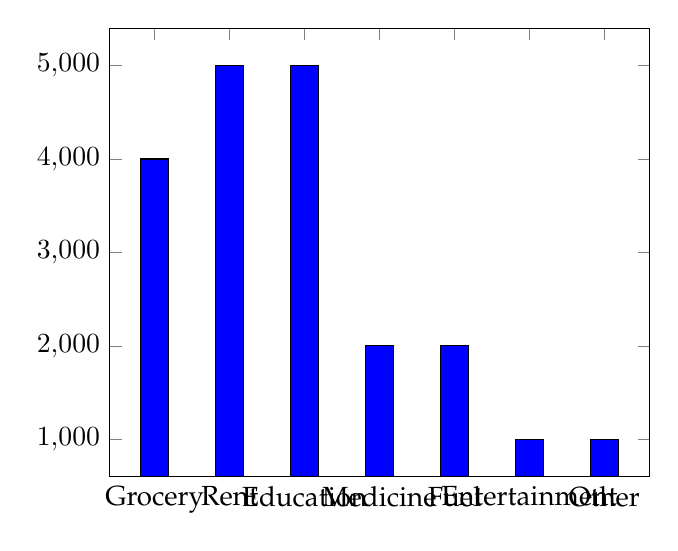
\begin{tikzpicture}
\begin{axis}[
    symbolic x coords={Grocery,Rent,Education,Medicine,Fuel,Entertainment,Other},
    xtick=data]
    \addplot[ybar,fill=blue] coordinates {
        (Grocery,4000)
        (Rent,5000)
        (Education,5000)
        (Medicine,2000)
        (Fuel,2000)
        (Entertainment,1000)
        (Other,1000)
    };
\end{axis}
\end{tikzpicture}
\end{center}

\end{document}